% Options for packages loaded elsewhere
\PassOptionsToPackage{unicode}{hyperref}
\PassOptionsToPackage{hyphens}{url}
\PassOptionsToPackage{dvipsnames,svgnames,x11names}{xcolor}
%
\documentclass[
  letterpaper,
  DIV=11,
  numbers=noendperiod]{scrartcl}

\usepackage{amsmath,amssymb}
\usepackage{iftex}
\ifPDFTeX
  \usepackage[T1]{fontenc}
  \usepackage[utf8]{inputenc}
  \usepackage{textcomp} % provide euro and other symbols
\else % if luatex or xetex
  \usepackage{unicode-math}
  \defaultfontfeatures{Scale=MatchLowercase}
  \defaultfontfeatures[\rmfamily]{Ligatures=TeX,Scale=1}
\fi
\usepackage{lmodern}
\ifPDFTeX\else  
    % xetex/luatex font selection
\fi
% Use upquote if available, for straight quotes in verbatim environments
\IfFileExists{upquote.sty}{\usepackage{upquote}}{}
\IfFileExists{microtype.sty}{% use microtype if available
  \usepackage[]{microtype}
  \UseMicrotypeSet[protrusion]{basicmath} % disable protrusion for tt fonts
}{}
\makeatletter
\@ifundefined{KOMAClassName}{% if non-KOMA class
  \IfFileExists{parskip.sty}{%
    \usepackage{parskip}
  }{% else
    \setlength{\parindent}{0pt}
    \setlength{\parskip}{6pt plus 2pt minus 1pt}}
}{% if KOMA class
  \KOMAoptions{parskip=half}}
\makeatother
\usepackage{xcolor}
\setlength{\emergencystretch}{3em} % prevent overfull lines
\setcounter{secnumdepth}{5}
% Make \paragraph and \subparagraph free-standing
\makeatletter
\ifx\paragraph\undefined\else
  \let\oldparagraph\paragraph
  \renewcommand{\paragraph}{
    \@ifstar
      \xxxParagraphStar
      \xxxParagraphNoStar
  }
  \newcommand{\xxxParagraphStar}[1]{\oldparagraph*{#1}\mbox{}}
  \newcommand{\xxxParagraphNoStar}[1]{\oldparagraph{#1}\mbox{}}
\fi
\ifx\subparagraph\undefined\else
  \let\oldsubparagraph\subparagraph
  \renewcommand{\subparagraph}{
    \@ifstar
      \xxxSubParagraphStar
      \xxxSubParagraphNoStar
  }
  \newcommand{\xxxSubParagraphStar}[1]{\oldsubparagraph*{#1}\mbox{}}
  \newcommand{\xxxSubParagraphNoStar}[1]{\oldsubparagraph{#1}\mbox{}}
\fi
\makeatother

\usepackage{color}
\usepackage{fancyvrb}
\newcommand{\VerbBar}{|}
\newcommand{\VERB}{\Verb[commandchars=\\\{\}]}
\DefineVerbatimEnvironment{Highlighting}{Verbatim}{commandchars=\\\{\}}
% Add ',fontsize=\small' for more characters per line
\usepackage{framed}
\definecolor{shadecolor}{RGB}{241,243,245}
\newenvironment{Shaded}{\begin{snugshade}}{\end{snugshade}}
\newcommand{\AlertTok}[1]{\textcolor[rgb]{0.68,0.00,0.00}{#1}}
\newcommand{\AnnotationTok}[1]{\textcolor[rgb]{0.37,0.37,0.37}{#1}}
\newcommand{\AttributeTok}[1]{\textcolor[rgb]{0.40,0.45,0.13}{#1}}
\newcommand{\BaseNTok}[1]{\textcolor[rgb]{0.68,0.00,0.00}{#1}}
\newcommand{\BuiltInTok}[1]{\textcolor[rgb]{0.00,0.23,0.31}{#1}}
\newcommand{\CharTok}[1]{\textcolor[rgb]{0.13,0.47,0.30}{#1}}
\newcommand{\CommentTok}[1]{\textcolor[rgb]{0.37,0.37,0.37}{#1}}
\newcommand{\CommentVarTok}[1]{\textcolor[rgb]{0.37,0.37,0.37}{\textit{#1}}}
\newcommand{\ConstantTok}[1]{\textcolor[rgb]{0.56,0.35,0.01}{#1}}
\newcommand{\ControlFlowTok}[1]{\textcolor[rgb]{0.00,0.23,0.31}{\textbf{#1}}}
\newcommand{\DataTypeTok}[1]{\textcolor[rgb]{0.68,0.00,0.00}{#1}}
\newcommand{\DecValTok}[1]{\textcolor[rgb]{0.68,0.00,0.00}{#1}}
\newcommand{\DocumentationTok}[1]{\textcolor[rgb]{0.37,0.37,0.37}{\textit{#1}}}
\newcommand{\ErrorTok}[1]{\textcolor[rgb]{0.68,0.00,0.00}{#1}}
\newcommand{\ExtensionTok}[1]{\textcolor[rgb]{0.00,0.23,0.31}{#1}}
\newcommand{\FloatTok}[1]{\textcolor[rgb]{0.68,0.00,0.00}{#1}}
\newcommand{\FunctionTok}[1]{\textcolor[rgb]{0.28,0.35,0.67}{#1}}
\newcommand{\ImportTok}[1]{\textcolor[rgb]{0.00,0.46,0.62}{#1}}
\newcommand{\InformationTok}[1]{\textcolor[rgb]{0.37,0.37,0.37}{#1}}
\newcommand{\KeywordTok}[1]{\textcolor[rgb]{0.00,0.23,0.31}{\textbf{#1}}}
\newcommand{\NormalTok}[1]{\textcolor[rgb]{0.00,0.23,0.31}{#1}}
\newcommand{\OperatorTok}[1]{\textcolor[rgb]{0.37,0.37,0.37}{#1}}
\newcommand{\OtherTok}[1]{\textcolor[rgb]{0.00,0.23,0.31}{#1}}
\newcommand{\PreprocessorTok}[1]{\textcolor[rgb]{0.68,0.00,0.00}{#1}}
\newcommand{\RegionMarkerTok}[1]{\textcolor[rgb]{0.00,0.23,0.31}{#1}}
\newcommand{\SpecialCharTok}[1]{\textcolor[rgb]{0.37,0.37,0.37}{#1}}
\newcommand{\SpecialStringTok}[1]{\textcolor[rgb]{0.13,0.47,0.30}{#1}}
\newcommand{\StringTok}[1]{\textcolor[rgb]{0.13,0.47,0.30}{#1}}
\newcommand{\VariableTok}[1]{\textcolor[rgb]{0.07,0.07,0.07}{#1}}
\newcommand{\VerbatimStringTok}[1]{\textcolor[rgb]{0.13,0.47,0.30}{#1}}
\newcommand{\WarningTok}[1]{\textcolor[rgb]{0.37,0.37,0.37}{\textit{#1}}}

\providecommand{\tightlist}{%
  \setlength{\itemsep}{0pt}\setlength{\parskip}{0pt}}\usepackage{longtable,booktabs,array}
\usepackage{calc} % for calculating minipage widths
% Correct order of tables after \paragraph or \subparagraph
\usepackage{etoolbox}
\makeatletter
\patchcmd\longtable{\par}{\if@noskipsec\mbox{}\fi\par}{}{}
\makeatother
% Allow footnotes in longtable head/foot
\IfFileExists{footnotehyper.sty}{\usepackage{footnotehyper}}{\usepackage{footnote}}
\makesavenoteenv{longtable}
\usepackage{graphicx}
\makeatletter
\newsavebox\pandoc@box
\newcommand*\pandocbounded[1]{% scales image to fit in text height/width
  \sbox\pandoc@box{#1}%
  \Gscale@div\@tempa{\textheight}{\dimexpr\ht\pandoc@box+\dp\pandoc@box\relax}%
  \Gscale@div\@tempb{\linewidth}{\wd\pandoc@box}%
  \ifdim\@tempb\p@<\@tempa\p@\let\@tempa\@tempb\fi% select the smaller of both
  \ifdim\@tempa\p@<\p@\scalebox{\@tempa}{\usebox\pandoc@box}%
  \else\usebox{\pandoc@box}%
  \fi%
}
% Set default figure placement to htbp
\def\fps@figure{htbp}
\makeatother

\KOMAoption{captions}{tableheading}
\makeatletter
\@ifpackageloaded{caption}{}{\usepackage{caption}}
\AtBeginDocument{%
\ifdefined\contentsname
  \renewcommand*\contentsname{Table of contents}
\else
  \newcommand\contentsname{Table of contents}
\fi
\ifdefined\listfigurename
  \renewcommand*\listfigurename{List of Figures}
\else
  \newcommand\listfigurename{List of Figures}
\fi
\ifdefined\listtablename
  \renewcommand*\listtablename{List of Tables}
\else
  \newcommand\listtablename{List of Tables}
\fi
\ifdefined\figurename
  \renewcommand*\figurename{Figure}
\else
  \newcommand\figurename{Figure}
\fi
\ifdefined\tablename
  \renewcommand*\tablename{Table}
\else
  \newcommand\tablename{Table}
\fi
}
\@ifpackageloaded{float}{}{\usepackage{float}}
\floatstyle{ruled}
\@ifundefined{c@chapter}{\newfloat{codelisting}{h}{lop}}{\newfloat{codelisting}{h}{lop}[chapter]}
\floatname{codelisting}{Stan

Program}
\newcommand*\listoflistings{\listof{codelisting}{List of Listings}}
\makeatother
\makeatletter
\makeatother
\makeatletter
\@ifpackageloaded{caption}{}{\usepackage{caption}}
\@ifpackageloaded{subcaption}{}{\usepackage{subcaption}}
\makeatother

\usepackage{bookmark}

\IfFileExists{xurl.sty}{\usepackage{xurl}}{} % add URL line breaks if available
\urlstyle{same} % disable monospaced font for URLs
\hypersetup{
  pdftitle={Constrained Transformations in Stan and Jax},
  pdfauthor={Michael Issa},
  colorlinks=true,
  linkcolor={blue},
  filecolor={Maroon},
  citecolor={Blue},
  urlcolor={Blue},
  pdfcreator={LaTeX via pandoc}}


\title{Constrained Transformations in Stan and Jax}
\author{Michael Issa}
\date{February 2025}

\begin{document}
\maketitle

\renewcommand*\contentsname{Table of contents}
{
\hypersetup{linkcolor=}
\setcounter{tocdepth}{3}
\tableofcontents
}

\section{General Setup}\label{general-setup}

\begin{Shaded}
\begin{Highlighting}[]
\ImportTok{import}\NormalTok{ matplotlib.pyplot }\ImportTok{as}\NormalTok{ plt}
\ImportTok{import}\NormalTok{ logging}
\ImportTok{import}\NormalTok{ cmdstanpy}
\ImportTok{from}\NormalTok{ cmdstanpy }\ImportTok{import}\NormalTok{ CmdStanModel}
\ImportTok{import}\NormalTok{ pandas }\ImportTok{as}\NormalTok{ pd}
\ImportTok{import}\NormalTok{ numpy }\ImportTok{as}\NormalTok{ np}
\ImportTok{import}\NormalTok{ warnings}
\ImportTok{import}\NormalTok{ arviz }\ImportTok{as}\NormalTok{ az}
\ImportTok{import}\NormalTok{ os}

\NormalTok{warnings.filterwarnings(}\StringTok{"ignore"}\NormalTok{)}

\CommentTok{\# Graphic configuration}
\NormalTok{c\_light }\OperatorTok{=} \StringTok{"\#DCBCBC"}
\NormalTok{c\_light\_highlight }\OperatorTok{=} \StringTok{"\#C79999"}
\NormalTok{c\_mid }\OperatorTok{=} \StringTok{"\#B97C7C"}
\NormalTok{c\_mid\_highlight }\OperatorTok{=} \StringTok{"\#A25050"}
\NormalTok{c\_dark }\OperatorTok{=} \StringTok{"\#8F2727"}
\NormalTok{c\_dark\_highlight }\OperatorTok{=} \StringTok{"\#7C0000"}

\NormalTok{c\_light\_teal }\OperatorTok{=} \StringTok{"\#6B8E8E"}
\NormalTok{c\_mid\_teal }\OperatorTok{=} \StringTok{"\#487575"}
\NormalTok{c\_dark\_teal }\OperatorTok{=} \StringTok{"\#1D4F4F"}

\NormalTok{RANDOM\_SEED }\OperatorTok{=} \DecValTok{58583389}
\NormalTok{np.random.seed(RANDOM\_SEED)}
\NormalTok{az.style.use(}\StringTok{"arviz{-}whitegrid"}\NormalTok{)}

\NormalTok{plt.rcParams[}\StringTok{\textquotesingle{}font.family\textquotesingle{}}\NormalTok{] }\OperatorTok{=} \StringTok{\textquotesingle{}serif\textquotesingle{}}

\NormalTok{plt.rcParams[}\StringTok{\textquotesingle{}xtick.labelsize\textquotesingle{}}\NormalTok{] }\OperatorTok{=} \DecValTok{12}
\NormalTok{plt.rcParams[}\StringTok{\textquotesingle{}ytick.labelsize\textquotesingle{}}\NormalTok{] }\OperatorTok{=} \DecValTok{12}
\NormalTok{plt.rcParams[}\StringTok{\textquotesingle{}axes.labelsize\textquotesingle{}}\NormalTok{] }\OperatorTok{=} \DecValTok{12}
\NormalTok{plt.rcParams[}\StringTok{\textquotesingle{}axes.titlesize\textquotesingle{}}\NormalTok{] }\OperatorTok{=} \DecValTok{12}

\NormalTok{plt.rcParams[}\StringTok{\textquotesingle{}axes.spines.top\textquotesingle{}}\NormalTok{] }\OperatorTok{=} \VariableTok{False}
\NormalTok{plt.rcParams[}\StringTok{\textquotesingle{}axes.spines.right\textquotesingle{}}\NormalTok{] }\OperatorTok{=} \VariableTok{False}
\NormalTok{plt.rcParams[}\StringTok{\textquotesingle{}axes.spines.left\textquotesingle{}}\NormalTok{] }\OperatorTok{=} \VariableTok{True}
\NormalTok{plt.rcParams[}\StringTok{\textquotesingle{}axes.spines.bottom\textquotesingle{}}\NormalTok{] }\OperatorTok{=} \VariableTok{True}

\NormalTok{plt.rcParams[}\StringTok{\textquotesingle{}axes.xmargin\textquotesingle{}}\NormalTok{] }\OperatorTok{=} \DecValTok{0}
\NormalTok{plt.rcParams[}\StringTok{\textquotesingle{}axes.ymargin\textquotesingle{}}\NormalTok{] }\OperatorTok{=} \DecValTok{0}

\NormalTok{plt.subplots\_adjust(left}\OperatorTok{=}\FloatTok{0.15}\NormalTok{, bottom}\OperatorTok{=}\FloatTok{0.15}\NormalTok{, right}\OperatorTok{=}\FloatTok{0.9}\NormalTok{, top}\OperatorTok{=}\FloatTok{0.85}\NormalTok{)}

\NormalTok{current\_working\_directory }\OperatorTok{=}\NormalTok{ os.getcwd()}

\NormalTok{cmdstanpy\_logger }\OperatorTok{=}\NormalTok{ logging.getLogger(}\StringTok{"cmdstanpy"}\NormalTok{)}
\NormalTok{cmdstanpy\_logger.disabled }\OperatorTok{=} \VariableTok{True}
\NormalTok{cmdstanpy.install\_cmdstan(compiler}\OperatorTok{=}\VariableTok{True}\NormalTok{)}
\end{Highlighting}
\end{Shaded}

\begin{verbatim}
CmdStan install directory: C:\Users\issam_biodcm6\.cmdstan
CmdStan version 2.36.0 already installed
Test model compilation
\end{verbatim}

\begin{verbatim}
True
\end{verbatim}

\begin{verbatim}
<Figure size 720x480 with 0 Axes>
\end{verbatim}

This is part 1 of a series of documents charting the progression of my
work on JaxGPStuff. I've always found it helpful to take the time to
write out the actual content of what a specific part of a program is
doing in a long-form cogent manner (something I think isn't done enough
if at all), and it's something I immensely appreciate (I don't enjoy
digging through your raw codebase to find out what you've done).

\section{Constrained Transformations in
Stan}\label{constrained-transformations-in-stan}

We'll start out easy with an example of in Stan and explain what it is
Stan is doing by constraining parameters.

First we'll simulate some simple regression data. In statistics and
maths, we have various constraints on some parameters values. Variances
or standard deviations must be positive, probabilities must be between 0
and 1, correlation matrices must have eigenvalues in valid ranges, etc.
Some of them we know are constrained to be positive because they are so
defined like the standard deviation. Other times we know, if these
parameters are being intepreted or are structured in some way, that
these parameters must be positive. Assume we don't already know what our
regression parameters values are, as we usually don't. But we have some
idea that they are positive because maybe the intercept stands for
average height and there are no negative height values so no negative
mean heights. This is a constraint imposed by the problem we're
studying.

\begin{Shaded}
\begin{Highlighting}[]
\ImportTok{from}\NormalTok{ sklearn.linear\_model }\ImportTok{import}\NormalTok{ LinearRegression}
\ImportTok{from}\NormalTok{ sklearn.metrics }\ImportTok{import}\NormalTok{ mean\_squared\_error}

\CommentTok{\# Simulate data}
\NormalTok{n }\OperatorTok{=} \DecValTok{100}      
\NormalTok{alpha }\OperatorTok{=} \DecValTok{2}        
\NormalTok{beta }\OperatorTok{=} \FloatTok{1.5}       
\NormalTok{sigma }\OperatorTok{=} \FloatTok{0.8}      

\NormalTok{x }\OperatorTok{=}\NormalTok{ np.random.normal(loc}\OperatorTok{=}\DecValTok{0}\NormalTok{, scale}\OperatorTok{=}\DecValTok{1}\NormalTok{, size}\OperatorTok{=}\NormalTok{n)}

\NormalTok{error }\OperatorTok{=}\NormalTok{ np.random.normal(loc}\OperatorTok{=}\DecValTok{0}\NormalTok{, scale}\OperatorTok{=}\NormalTok{sigma, size}\OperatorTok{=}\NormalTok{n)}
\NormalTok{y }\OperatorTok{=}\NormalTok{ alpha }\OperatorTok{+}\NormalTok{ beta }\OperatorTok{*}\NormalTok{ x }\OperatorTok{+}\NormalTok{ error}

\NormalTok{sim\_data }\OperatorTok{=}\NormalTok{ pd.DataFrame(\{}\StringTok{\textquotesingle{}x\textquotesingle{}}\NormalTok{: x, }\StringTok{\textquotesingle{}y\textquotesingle{}}\NormalTok{: y\})}

\NormalTok{x\_reshaped }\OperatorTok{=}\NormalTok{ x.reshape(}\OperatorTok{{-}}\DecValTok{1}\NormalTok{, }\DecValTok{1}\NormalTok{)  }
\NormalTok{model }\OperatorTok{=}\NormalTok{ LinearRegression()}
\NormalTok{model.fit(x\_reshaped, y)}

\BuiltInTok{print}\NormalTok{(}\StringTok{"Intercept (alpha):"}\NormalTok{, model.intercept\_)}
\BuiltInTok{print}\NormalTok{(}\StringTok{"Coefficient (beta):"}\NormalTok{, model.coef\_[}\DecValTok{0}\NormalTok{])}
\BuiltInTok{print}\NormalTok{(}\StringTok{"Mean squared error:"}\NormalTok{, mean\_squared\_error(y, model.predict(x\_reshaped)))}

\NormalTok{plt.scatter(x, y, label}\OperatorTok{=}\StringTok{"Simulated data"}\NormalTok{, alpha}\OperatorTok{=}\FloatTok{0.7}\NormalTok{, color}\OperatorTok{=}\NormalTok{c\_mid\_highlight)}
\NormalTok{plt.plot(x, alpha }\OperatorTok{+}\NormalTok{ beta }\OperatorTok{*}\NormalTok{ x, color}\OperatorTok{=}\StringTok{"black"}\NormalTok{, label}\OperatorTok{=}\StringTok{"True regression line"}\NormalTok{, linewidth}\OperatorTok{=}\DecValTok{2}\NormalTok{)}
\NormalTok{plt.xlabel(}\StringTok{"x"}\NormalTok{)}
\NormalTok{plt.ylabel(}\StringTok{"y"}\NormalTok{)}
\NormalTok{plt.title(}\StringTok{"Simulated Regression Data"}\NormalTok{)}
\NormalTok{plt.legend(loc}\OperatorTok{=}\StringTok{"upper left"}\NormalTok{)}
\NormalTok{plt.show()}
\end{Highlighting}
\end{Shaded}

\begin{verbatim}
Intercept (alpha): 1.8796387702452613
Coefficient (beta): 1.5259117159172857
Mean squared error: 0.6303553871943935
\end{verbatim}

\pandocbounded{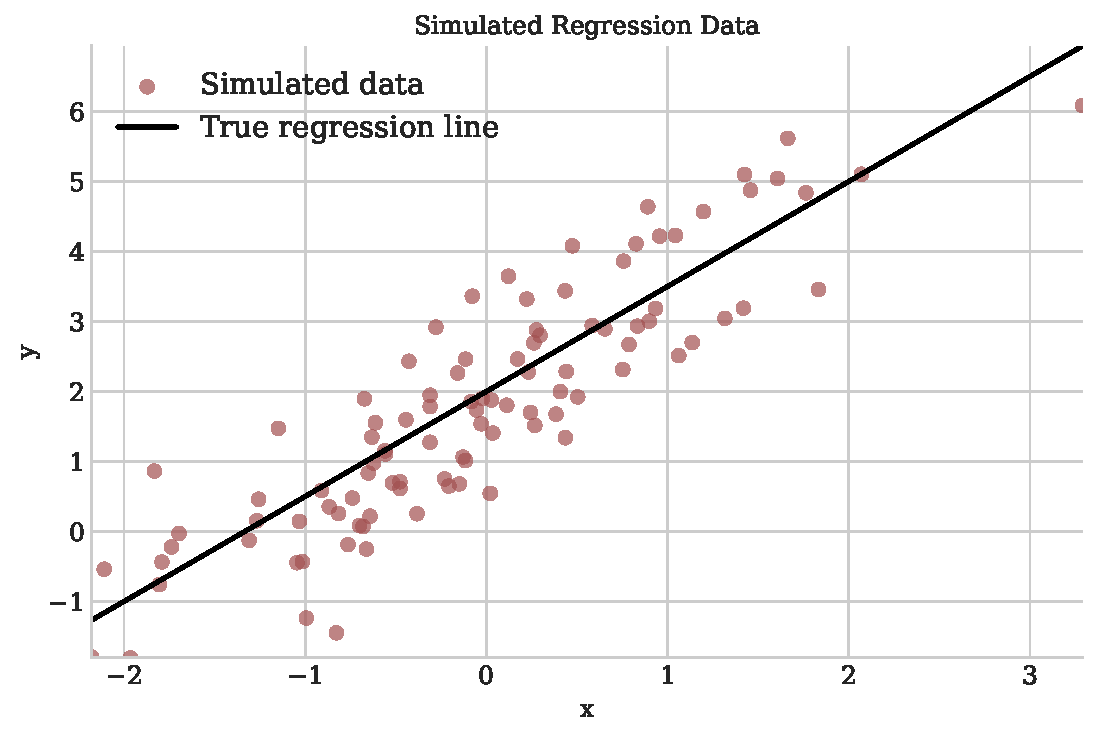
\includegraphics[keepaspectratio]{transforms_files/figure-pdf/cell-3-output-2.pdf}}

In Stan, we specify constraints in various ways (see the
\href{https://mc-stan.org/docs/reference-manual/types.html\#variable-declaration.section}{variables
declaration} section for the syntax specification) but typically you'll
see \textless lower=0\textgreater{} following the function argument
type. This expresses a constraint of positivity on whatever parameter it
attaches to. Here's a Stan model used to fit our simulated data that
uses it for all parameter delcarations.

\begin{codelisting}

\caption{\texttt{model1.stan}}

\begin{Shaded}
\begin{Highlighting}[]
\KeywordTok{data}\NormalTok{ \{}
    \DataTypeTok{int}\NormalTok{\textless{}}\KeywordTok{lower}\NormalTok{=}\DecValTok{0}\NormalTok{\textgreater{} N;}
    \DataTypeTok{vector}\NormalTok{[N] x;}
    \DataTypeTok{vector}\NormalTok{[N] y;}
\NormalTok{\}}

\KeywordTok{parameters}\NormalTok{ \{}
    \DataTypeTok{real}\NormalTok{\textless{}}\KeywordTok{lower}\NormalTok{=}\DecValTok{0}\NormalTok{\textgreater{} alpha;}
    \DataTypeTok{real}\NormalTok{\textless{}}\KeywordTok{lower}\NormalTok{=}\DecValTok{0}\NormalTok{\textgreater{} beta;}
    \DataTypeTok{real}\NormalTok{\textless{}}\KeywordTok{lower}\NormalTok{=}\DecValTok{0}\NormalTok{\textgreater{} sigma; }
\NormalTok{\}}

\KeywordTok{model}\NormalTok{ \{}
\NormalTok{    y \textasciitilde{} normal(alpha + beta * x, sigma);  }
\NormalTok{\}}
\end{Highlighting}
\end{Shaded}

\end{codelisting}

Now, it's quite opaque what exactly the constraints are doing here when
the computation occurs, but we can explictly represent the constraints
Stan computes using the simple transformations Stan is using under the
hood. Here is the model without the constraint syntax but constrained by
explicit syntactic representation of the computation and by updating the
log probability manually.

\begin{codelisting}

\caption{\texttt{model1\_explicit.stan}}

\begin{Shaded}
\begin{Highlighting}[]
\KeywordTok{data}\NormalTok{ \{}
    \DataTypeTok{int}\NormalTok{\textless{}}\KeywordTok{lower}\NormalTok{=}\DecValTok{0}\NormalTok{\textgreater{} N;}
    \DataTypeTok{vector}\NormalTok{[N] x;}
    \DataTypeTok{vector}\NormalTok{[N] y;}
\NormalTok{\}}

\KeywordTok{parameters}\NormalTok{ \{}
    \DataTypeTok{real}\NormalTok{ alpha\_unc; }
    \DataTypeTok{real}\NormalTok{ beta\_unc;}
    \DataTypeTok{real}\NormalTok{ sigma\_unc;}
\NormalTok{\}}

\KeywordTok{transformed parameters}\NormalTok{ \{}
    \DataTypeTok{real}\NormalTok{ alpha = exp(alpha\_unc); }
    \DataTypeTok{real}\NormalTok{ beta = exp(beta\_unc);   }
    \DataTypeTok{real}\NormalTok{ sigma = exp(sigma\_unc); }
\NormalTok{\}}

\KeywordTok{model}\NormalTok{ \{}
    \KeywordTok{target +=}\NormalTok{ alpha\_unc;  }
    \KeywordTok{target +=}\NormalTok{ beta\_unc;  }
    \KeywordTok{target +=}\NormalTok{ sigma\_unc;  }
    
\NormalTok{    y \textasciitilde{} normal(alpha + beta * x, sigma);}
\NormalTok{\}}
\end{Highlighting}
\end{Shaded}

\end{codelisting}

We fit both our models and look at the output summary now.

\begin{Shaded}
\begin{Highlighting}[]
\NormalTok{data }\OperatorTok{=}\NormalTok{ \{}
    \StringTok{\textquotesingle{}N\textquotesingle{}}\NormalTok{: n,}
    \StringTok{\textquotesingle{}x\textquotesingle{}}\NormalTok{: x.tolist(),}
    \StringTok{\textquotesingle{}y\textquotesingle{}}\NormalTok{: y.tolist(),}
\NormalTok{\}}
\end{Highlighting}
\end{Shaded}

\begin{Shaded}
\begin{Highlighting}[]
\NormalTok{model1 }\OperatorTok{=}\NormalTok{ CmdStanModel(stan\_file}\OperatorTok{=}\StringTok{\textquotesingle{}models/model1.stan\textquotesingle{}}\NormalTok{)}
\NormalTok{fit1 }\OperatorTok{=}\NormalTok{ model1.sample(data}\OperatorTok{=}\NormalTok{data, chains}\OperatorTok{=}\DecValTok{4}\NormalTok{, iter\_sampling}\OperatorTok{=}\DecValTok{1000}\NormalTok{, iter\_warmup}\OperatorTok{=}\DecValTok{500}\NormalTok{, show\_progress}\OperatorTok{=}\VariableTok{False}\NormalTok{)}

\NormalTok{fit1.summary()}
\end{Highlighting}
\end{Shaded}

\begin{longtable}[]{@{}lllllllllll@{}}
\toprule\noalign{}
& Mean & MCSE & StdDev & MAD & 5\% & 50\% & 95\% & ESS\_bulk & ESS\_tail
& R\_hat \\
\midrule\noalign{}
\endhead
\bottomrule\noalign{}
\endlastfoot
lp\_\_ & -27.548300 & 0.026476 & 1.198950 & 0.964209 & -29.837700 &
-27.240700 & -26.259800 & 2147.79 & 2558.97 & 1.003560 \\
alpha & 1.879680 & 0.001388 & 0.079960 & 0.078289 & 1.746770 & 1.878510
& 2.011470 & 3346.63 & 2709.65 & 0.999894 \\
beta & 1.525990 & 0.001338 & 0.079584 & 0.076391 & 1.393150 & 1.525290 &
1.657350 & 3544.73 & 2811.84 & 1.003250 \\
sigma & 0.813226 & 0.000993 & 0.057706 & 0.055225 & 0.724179 & 0.809241
& 0.914189 & 3491.32 & 2747.22 & 1.000190 \\
\end{longtable}

\begin{Shaded}
\begin{Highlighting}[]
\NormalTok{model1\_explicit }\OperatorTok{=}\NormalTok{ CmdStanModel(stan\_file}\OperatorTok{=}\StringTok{\textquotesingle{}models//model1\_explicit.stan\textquotesingle{}}\NormalTok{)}
\NormalTok{fit2 }\OperatorTok{=}\NormalTok{ model1\_explicit.sample(data}\OperatorTok{=}\NormalTok{data, chains}\OperatorTok{=}\DecValTok{4}\NormalTok{, iter\_sampling}\OperatorTok{=}\DecValTok{1000}\NormalTok{, iter\_warmup}\OperatorTok{=}\DecValTok{500}\NormalTok{, show\_progress}\OperatorTok{=}\VariableTok{False}\NormalTok{)}

\NormalTok{fit2.summary()}
\end{Highlighting}
\end{Shaded}

\begin{longtable}[]{@{}lllllllllll@{}}
\toprule\noalign{}
& Mean & MCSE & StdDev & MAD & 5\% & 50\% & 95\% & ESS\_bulk & ESS\_tail
& R\_hat \\
\midrule\noalign{}
\endhead
\bottomrule\noalign{}
\endlastfoot
lp\_\_ & -27.591200 & 0.027615 & 1.224010 & 0.990822 & -30.099600 &
-27.270100 & -26.264700 & 1983.21 & 2941.93 & 1.00133 \\
alpha\_unc & 0.629911 & 0.000751 & 0.042230 & 0.041859 & 0.558216 &
0.631891 & 0.696182 & 3311.64 & 2410.25 & 1.00041 \\
beta\_unc & 0.420838 & 0.000920 & 0.054107 & 0.053601 & 0.329447 &
0.422932 & 0.508122 & 3538.02 & 2529.52 & 1.00040 \\
sigma\_unc & -0.209985 & 0.001252 & 0.071872 & 0.071369 & -0.326586 &
-0.210925 & -0.089854 & 3311.98 & 2626.49 & 1.00020 \\
alpha & 1.879110 & 0.001392 & 0.079052 & 0.078400 & 1.747550 & 1.881160
& 2.006080 & 3311.64 & 2410.25 & 1.00041 \\
beta & 1.525460 & 0.001388 & 0.082199 & 0.081291 & 1.390200 & 1.526430 &
1.662170 & 3538.04 & 2529.52 & 1.00038 \\
sigma & 0.812696 & 0.001027 & 0.058660 & 0.057593 & 0.721382 & 0.809835
& 0.914065 & 3312.01 & 2626.49 & 1.00015 \\
\end{longtable}

We see the two Stan models provided are mathematically equivalent and
will recover the same parameter values because they involve two closely
identical computations of the same reparameterization, a constrain of
positivity. The key difference between them lies in where the code is
being represented. Stan does it somewhere else as a subroutine not
represented to the user, but we did it directly. We'll break the math
down in a bit more detail now.

In the first model, the parameters \(\alpha\), \(\beta\), \(\sigma\) are
constrained to be greater than or equal to 0 (i.e., \(\alpha\),
\(\beta\), and \(\sigma\) \(\geq\) \(0\)). This means the model
explicitly ensures these parameters are non-negative during sampling.

Stan will sample these parameters directly in their constrained space
(keep in mind: sampling in the constrained space is NOT equivalent to
sampling and transforming your sample to be constrained. We'll revisit
this below). The parameter values are bounded between \(0\) and
\(\infty\). This means the likelihood will incorporate the probability
of the parameters being within the defined range, i.e., using the normal
distribution for the regression model, along with the boundary
conditions on the parameters (such as \(\sigma \geq 0\) ).

Both models are mathematically{[}\^{}1{]} equivalent because the
transformations in the second model enforce the same constraints on the
parameters as the first model but instead of performing the adjustment
on the log density automatically as Stan does if you specify bounds, we
do it by hand (Why increment the target probability by the value
\(X_{unc}\) you might ask? Keep reading). The transformation \(\exp(x)\)
maps all real values of \(\alpha_{\text{unc}}\), \(\beta_{\text{unc}}\),
and \(\sigma_{\text{unc}}\) to positive values, which is what the first
model does by directly imposing constraints
\(\alpha, \beta, \sigma \geq 0\).

\begin{itemize}
\tightlist
\item
  In the first model, the parameter space is constrained to be
  non-negative directly, so Stan only samples within the range
  \([0, \infty]\).
\item
  In the second model, the parameters are unconstrained, and the
  exponential transformation ensures that the resulting parameters are
  positive. The log of the Jacobian
  \(\log \left( \left| \frac{d}{dx} \exp(x) \right| \right)\) is then
  added to the target log-probability to adjust for the transformation
  from unconstrained space to constrained space because we want to
  interpret our sampling in the original space.
\end{itemize}

Both methods perform close to identical operations{[}\^{}2{]} for the
log densities and will therefore produce the same parameter values after
sampling. This is because both models are doing the same
reparameterization.

More precisely, the likelihood function in both models is:

\[
y_i \sim \mathcal{N}(\alpha + \beta x_i, \sigma)
\]

In the second model, the unconstrained parameters
\(\alpha_{\text{unc}}, \beta_{\text{unc}}, \sigma_{\text{unc}}\) are
mapped to positive values via the exponential function:

\[
\alpha = \exp(\alpha_{\text{unc}}), \quad \beta = \exp(\beta_{\text{unc}}), \quad \sigma = \exp(\sigma_{\text{unc}})
\]

The Jacobian of this transformation is:

\[
\frac{d}{d\theta} \exp(\theta) = \exp(\theta)
\]

So, the log-Jacobian adjustment is:

\[
\log(\exp(\alpha_{\text{unc}})) = \alpha_{\text{unc}}, \quad \log(\exp(\beta_{\text{unc}})) = \beta_{\text{unc}}, \quad \log(\exp(\sigma_{\text{unc}})) = \sigma_{\text{unc}}
\]

Thus, the log-probability is adjusted by adding these terms to account
for the transformation from the unconstrained space to the constrained
space. Stan typically does these change of variable transformations
automatically using a more generalized transformation for the
lower-bound constraint. But I find it quite nice that Stan allows you to
program things manually and increment the log density using target+=.
You might ask why would I ever care to figure out what the log Jacobian
adjustment is when Stan can do it for me?{[}\^{}3{]} You don't ever need
to if all you're doing is specifying constraints like the ones Stan
provides for variables, but there are constraints that you would want to
impose that do require it. There are too many reasons you'd want to that
I'm unaware of but here are a few: high posterior correlation in
unconstrained space (cf.~Neal's funnel), numerical stability, prior
stability, and sampling efficiency. It would take too long to go into
the details and Google is your best friend. Outside of Bayesian
inference related things, constrained transformation have found a home
in some kick ass generative models that are based on Normalizing
Flows.\footnote{Again Google.}

\section{A note on change of variables transformation vs
transformations}\label{a-note-on-change-of-variables-transformation-vs-transformations}

Smarter people than I have tried to drill this distinction. I highly,
highly recommend reading and rereading the Stan documentation
\href{https://mc-stan.org/docs/stan-users-guide/reparameterization.html\#change-of-variables.chapter}{here}.
They give many examples at varying complexity and really hammer home the
difference.

To put it succietnly, change of variables transformation are
transformations that first transform the variables AND THEN sample them.
Whereas transformations are typically taken to be instances where we
sample some variables AND THEN apply a functional transformation to
them. Again, read that Stan article. It provides many examples that
demonstrate the difference.

{[}\^{}1{]} NOT COMPUTATIONALLY EQUIVALENT.

{[}\^{}2{]} Not exactly.
\href{https://mc-stan.org/docs/reference-manual/transforms.html\#lower-bound-transform.section}{Stan
uses the general transformation} \(X = \exp(Y) + a\) for a lower bound
constraint being \(a\).

{[}\^{}3{]} Besides the fact that it's nice to know you can do it and
you should know what Stan is doing!

It would defeat the purpose if they were, and the transformation defines
a probability density, which is a non-unique, parameterization-dependent
function in \(\mathbb{R}^N \to \mathbb{R}_+\). In practice, this means a
given model can be represented different ways, and different
representations have different computational performances.




\end{document}
